\documentclass[11pt]{article}

\usepackage[margin=1in]{geometry}
\usepackage{amsmath,amssymb}
\usepackage{booktabs}
\usepackage{longtable}
\usepackage{xcolor}
\usepackage{enumitem}
\usepackage{tikz}
\usetikzlibrary{arrows.meta,positioning,calc,fit,backgrounds}
\usepackage{graphicx}
\usepackage{float}
\usepackage[hidelinks]{hyperref}
\usepackage[htt]{hyphenat}
\emergencystretch=2em

\definecolor{cardblue}{HTML}{2166AC}
\definecolor{evgreen}{HTML}{1B7837}
\definecolor{harmred}{HTML}{B2182B}
\definecolor{coldgray}{HTML}{7F7F7F}

\newcommand{\code}[1]{\texttt{\small #1}}
\newcommand{\gain}{g}
\newcommand{\card}{c}
\newcommand{\Beta}{\mathrm{Beta}}

\title{\textbf{GigaEvo Memory: How a Card Earns Its Place in the Prompt}\\[2pt]
\large Reputation from gain events, expected value, and the Thompson auction}
\author{GigaEvo --- \code{gigaevo/memory/read}}
\date{Rebuilt memory subsystem (PR \#294, branch \code{refactor/memory-rebuild})}

\begin{document}
\maketitle

\begin{abstract}
The read side of GigaEvo memory decides, for one mutation, \emph{which} previously
banked cards (insights or exemplar programs) --- if any --- to inject into the
mutator's prompt. This document traces the full chain of arithmetic behind that
decision: how a card's \emph{gain events} (its measured effect on past children)
are collapsed into a \emph{reputation} (a Beta downside posterior plus a magnitude),
how reputation and magnitude combine into an \emph{expected value}, how a Thompson
auction pits each card against an ``inject nothing'' baseline arm, and how a budget
cap and renderer turn auction winners into prompt text. Every formula below is
grounded verbatim in \code{gigaevo/memory/read/reputation.py},
\code{read/auction.py}, \code{read/render.py}, and \code{write/stats.py}. It is the
companion to \emph{``How a Run Becomes a Card''} (the write-side report), which
authors the cards and produces the gain events this document consumes; the two
meet at the gain event.
\end{abstract}

\section*{Terminology}
\addcontentsline{toc}{section}{Terminology}

The read side borrows its vocabulary from multi-armed bandits and Bayesian
statistics. Every term below is defined here at first use and reused unchanged
throughout.

\begingroup
\setlength{\parskip}{0pt}
\begin{description}[leftmargin=1.4em, itemsep=1.5pt, parsep=0pt, style=unboxed]
  \item[\textcolor{cardblue}{Card}] a banked memory item --- either an
    \emph{insight} (a reusable text lesson) or an \emph{exemplar program} (a strong
    past solution). The unit that competes for a place in the prompt.
  \item[\textcolor{cardblue}{Gain event}] one record of how a card affected a past
    child: the signed, orientation-corrected fitness change of the child relative to
    the \emph{base parent} that card was helping to mutate (\S\ref{sec:gain}). A card's
    whole track record is its list of gain events.
  \item[\textcolor{cardblue}{Base parent}] the specific parent a child was anchored
    to and measured against. Under multi-parent mutation ``the parent'' is ambiguous,
    so the mutator names one (a 1-based index, first parent if out of range); a gain
    event's change is always child \emph{minus this base}, never another parent. The
    write-side report (\S2) covers how it is frozen at birth; here it is simply the
    baseline every gain is relative to.
  \item[\textcolor{evgreen}{Reputation}] a card's summarized track record ---
    a \emph{posterior} over how reliably it helps, plus a \emph{magnitude} for how
    much. Not a pipeline stage but the scoring function the auction consults.
  \item[\textcolor{evgreen}{Posterior}] the Bayesian distribution $\Beta(a,b)$ over
    a card's unknown \emph{help-probability} $\theta$, updated from its gain events.
    A wide posterior means ``uncertain''; a posterior mass near $1$ means
    ``reliably helpful''.
  \item[\textcolor{evgreen}{Magnitude $M$}] the typical \emph{size} of a card's
    effect --- the signed median of its gains. The posterior says how
    \emph{reliably} a card helps; $M$ says how \emph{much} (and, by its sign,
    whether it helps at all).
  \item[\textcolor{harmred}{Arm}] bandit term for one selectable option. Here each
    candidate card is an arm, and they all compete against one virtual
    \emph{baseline arm} that represents ``inject nothing'' (leave the prompt as is).
  \item[\textcolor{harmred}{Thompson sampling}] a selection rule: draw one random
    sample from each arm's posterior and act on the best draw. It explores in
    proportion to uncertainty --- an under-tested card can still win on a lucky draw,
    a well-tested weak card almost never does.
  \item[\textcolor{harmred}{Gate ($\theta>\theta_0$)}] the reliability test inside
    the auction: a card's sampled help-probability $\theta$ must beat the baseline
    arm's sample $\theta_0$ on this draw to be eligible.
  \item[\textcolor{harmred}{Bid / expected value (EV)}] a card's score in the EV
    auction, $\tilde\theta\cdot\hat M$ --- a reliability draw scaled by effect size.
    A negative-magnitude card bids negative and is refused (\S\ref{sec:ev}).
  \item[\textcolor{cardblue}{Shortlist (slate)}] the $\le 10$ cards retrieval
    surfaces for one decision --- the \emph{population} the auction ranks. (In the
    bandit literature the set of options offered together is a \emph{slate}.)
  \item[\textcolor{cardblue}{Candidate}] a shortlisted card wrapped with its
    posterior $(a,b)$ and magnitude $M$ for the auction (\code{AuctionCandidate}).
  \item[\textcolor{cardblue}{Budget}] the cap on how many auction winners are
    actually rendered into the prompt --- one slot by default
    (\code{reader.max\_cards}, \S\ref{sec:round}).
  \item[\textcolor{coldgray}{Cold card}] a card with \emph{no} gain events (or a
    corrupt/absent stamped posterior); its posterior falls back to the uniform prior
    $\Beta(1,1)$ and it rides an exploration coin-flip rather than an earned
    reputation. Note this is stricter than ``few'': even one event yields a real
    posterior --- a single win gives $\Beta(2,1)$, not $\Beta(1,1)$. The
    \code{harm\_min\_events}${=}3$ floor is a separate gate on \emph{eviction}, not
    on whether a card is cold.
  \item[\textcolor{coldgray}{Cell (behavioral descriptor)}] a MAP-Elites bucket of
    the search space. BD-proximity reputation restricts a card's evidence to the
    gain events whose parents share the \emph{query} parent's cell (\S\ref{sec:bd}).
\end{description}
\endgroup

\section{The read pipeline at a glance}

For each mutation the reader runs a five-stage funnel
(\code{read/reader.py}, \code{MemoryReader.\_select}). Figure~\ref{fig:flow}
shows the whole system: an \emph{evidence tier} (top) turns the card bank and the
program pool into a per-card reputation, and a \emph{reader tier} (bottom) spends
that reputation to fill a single prompt slot.

\begin{figure}[ht]
\centering
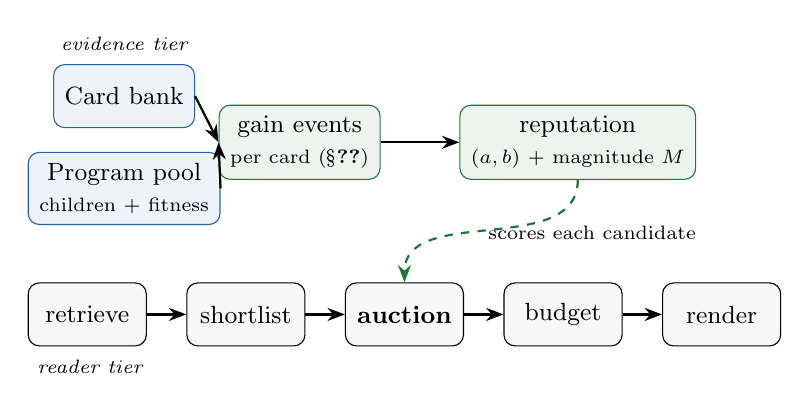
\begin{tikzpicture}[
  font=\small,
  box/.style={draw, rounded corners, align=center, inner sep=4pt, minimum height=8mm},
  src/.style={box, fill=cardblue!8, draw=cardblue},
  ev/.style={box, fill=evgreen!8, draw=evgreen},
  st/.style={box, minimum width=15mm, fill=black!3},
  arr/.style={-{Stealth[length=2.2mm]}, thick},
  darr/.style={-{Stealth[length=2.2mm]}, thick, dashed, draw=evgreen}]
% evidence tier
\node[src] (bank) {Card bank};
\node[src, below=3mm of bank] (pool) {Program pool\\{\scriptsize children $+$ fitness}};
\node[ev, right=12mm of $(bank)!0.5!(pool)$] (ge)
  {gain events\\{\scriptsize per card (\S\ref{sec:gain})}};
\node[ev, right=10mm of ge] (rep)
  {reputation\\{\scriptsize $(a,b)$ + magnitude $M$}};
\draw[arr] (bank.east) -- (ge.west);
\draw[arr] (pool.east) -- (ge.west);
\draw[arr] (ge) -- (rep);
% reader tier
\node[st, below=16mm of pool.west, anchor=west] (ret) {retrieve};
\node[st, right=5mm of ret] (sh) {shortlist};
\node[st, right=5mm of sh] (au) {\textbf{auction}};
\node[st, right=5mm of au] (bu) {budget};
\node[st, right=5mm of bu] (rn) {render};
\draw[arr] (ret)--(sh); \draw[arr] (sh)--(au);
\draw[arr] (au)--(bu); \draw[arr] (bu)--(rn);
\draw[darr] (rep.south) to[out=-90,in=90] node[right,font=\scriptsize,pos=0.55]
  {scores each candidate} (au.north);
\node[font=\scriptsize, above=0.5mm of bank] {\itshape evidence tier};
\node[font=\scriptsize, below=0.5mm of ret.south west, anchor=north west] {\itshape reader tier};
\end{tikzpicture}
\caption{The memory read system. Reputation is not a pipeline stage --- it is the
\emph{scoring function} the auction consults. Every card surviving the shortlist
becomes an \code{AuctionCandidate} carrying its posterior $(a,b)$ and signed
magnitude $M$, both read from that card's gain events at decision time.}
\label{fig:flow}
\end{figure}

\paragraph{Three funnel widths.} Three distinct caps control how wide the funnel
is at each point; conflating them is the most common source of confusion.

\begin{center}
\begin{tabular}{@{}lll@{}}
\toprule
Width & Config key & Default (shipped \code{full}/\code{reader}) \\
\midrule
Retrieval fan-out (per query, per scope) & \code{research.default\_top\_k} & 10 \\
Recall shortlist (auction population)     & \code{research.max\_cards}     & 10 \\
Injection budget (winners rendered)       & \code{reader.max\_cards}       & 1 \\
\bottomrule
\end{tabular}
\end{center}

So up to ten cards reach the auction, but at most \emph{one} is ever written into
the prompt (Figure~\ref{fig:funnel}). The auction's job is to decide whether that
one slot is worth spending at all, and on which card.

\begin{figure}[ht]
\centering
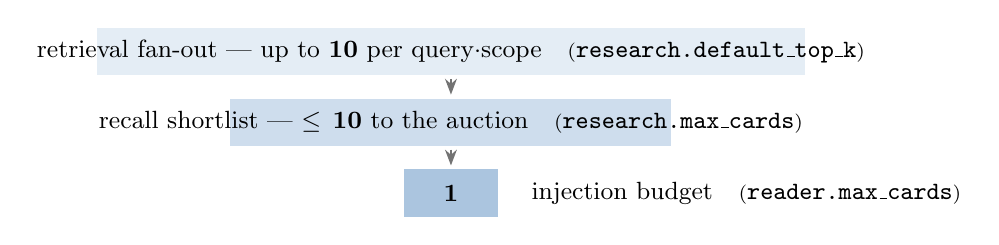
\begin{tikzpicture}[font=\small]
\fill[cardblue!12] (0,2.1) rectangle (9,2.7);
\node at (4.5,2.4) {retrieval fan-out --- up to \textbf{10} per query$\cdot$scope
  \ \ {\scriptsize(\code{research.default\_top\_k})}};
\fill[cardblue!22] (1.7,1.2) rectangle (7.3,1.8);
\node at (4.5,1.5) {recall shortlist --- $\le\,\textbf{10}$ to the auction
  \ \ {\scriptsize(\code{research.max\_cards})}};
\fill[cardblue!38] (3.9,0.3) rectangle (5.1,0.9);
\node at (4.5,0.6) {\textbf{1}};
\node[anchor=west] at (5.4,0.6) {injection budget
  \ \ {\scriptsize(\code{reader.max\_cards})}};
\draw[-{Stealth[length=2mm]}, thick, black!55] (4.5,2.05) -- (4.5,1.85);
\draw[-{Stealth[length=2mm]}, thick, black!55] (4.5,1.15) -- (4.5,0.95);
\end{tikzpicture}
\caption{Three funnel widths. The retrieval fan-out and the recall shortlist are
both wide (10); the injection budget is a single slot. Conflating these three caps
is the most common source of confusion.}
\label{fig:funnel}
\end{figure}

\section{From idea context and gains to a decision: the transformation}
\label{sec:transform}

Before the per-stage detail, Figure~\ref{fig:transform} walks one card end to end:
its idea context and raw gain events are transformed --- by a sign test, a
Beta posterior, a Thompson draw, and a baseline comparison --- into a single
auction decision and a line of prompt text. Every later section
(\S\ref{sec:gain}--\S\ref{sec:auction}, and \S\ref{sec:render} for the final
box) zooms into one arrow of this chain.

\begin{figure}[t]
\centering
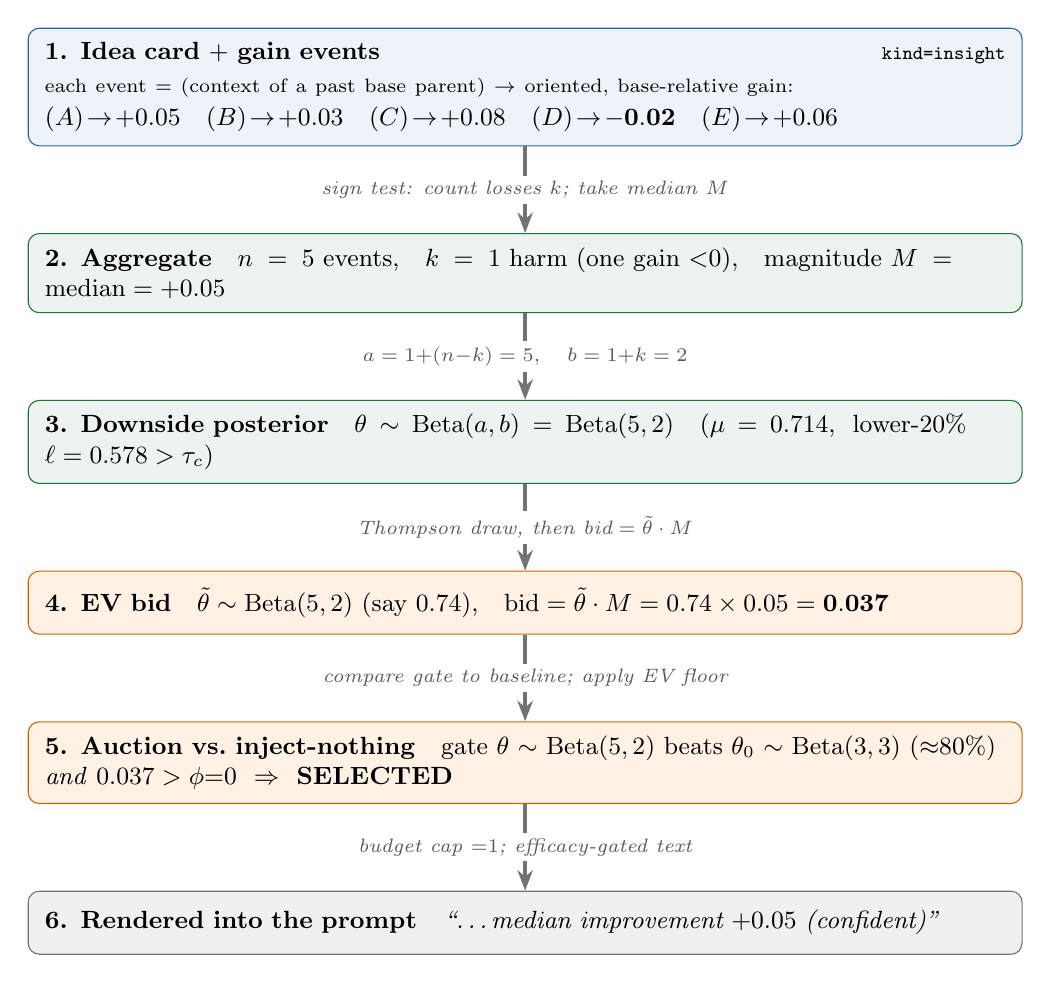
\begin{tikzpicture}[
  font=\small,
  stage/.style={draw, rounded corners, align=left, inner xsep=6pt, inner ysep=5pt,
                text width=122mm, minimum height=8mm},
  op/.style={midway, fill=white, inner sep=2pt, font=\scriptsize\itshape,
             text=black!65},
  a/.style={-{Stealth[length=2.6mm]}, very thick, draw=black!55}]
\node[stage, fill=cardblue!8, draw=cardblue] (raw)
  {\textbf{1. Idea card $+$ gain events} \hfill {\scriptsize\ttfamily kind=insight}\\[1pt]
   {\scriptsize each event $=$ (context of a past base parent) $\to$ oriented,
   base-relative gain:}\\[1pt]
   $(A)\!\to\!{+}0.05\quad (B)\!\to\!{+}0.03\quad (C)\!\to\!{+}0.08\quad
    (D)\!\to\!\mathbf{{-}0.02}\quad (E)\!\to\!{+}0.06$};
\node[stage, fill=evgreen!8, draw=evgreen, below=11mm of raw] (agg)
  {\textbf{2. Aggregate}\quad $n=5$ events,\quad
   $k=1$ harm (one gain ${<}0$),\quad
   magnitude $M=\operatorname{median}={+}0.05$};
\node[stage, fill=evgreen!8, draw=evgreen, below=11mm of agg] (post)
  {\textbf{3. Downside posterior}\quad
   $\theta\sim\Beta(a,b)=\Beta(5,2)$\quad
   ($\mu=0.714$,\ \ lower-20\% $\ell=0.578>\tau_c$)};
\node[stage, fill=orange!10, draw=orange!80!black, below=11mm of post] (bid)
  {\textbf{4. EV bid}\quad
   $\tilde\theta\sim\Beta(5,2)$ (say $0.74$),\quad
   $\text{bid}=\tilde\theta\cdot M=0.74\times0.05=\mathbf{0.037}$};
\node[stage, fill=orange!10, draw=orange!80!black, below=11mm of bid] (auc)
  {\textbf{5. Auction vs.\ inject-nothing}\quad
   gate $\theta\sim\Beta(5,2)$ beats $\theta_0\sim\Beta(3,3)$ ($\approx$80\%)
   \emph{and} $0.037>\phi{=}0$\ \ $\Rightarrow$\ \ \textbf{SELECTED}};
\node[stage, fill=black!6, draw=black!55, below=11mm of auc] (out)
  {\textbf{6. Rendered into the prompt}\quad
   \emph{``\ldots median improvement ${+}0.05$ (confident)''}};
\draw[a] (raw) -- (agg) node[op]{sign test: count losses $k$; take median $M$};
\draw[a] (agg) -- (post) node[op]{$a=1{+}(n{-}k)=5,\quad b=1{+}k=2$};
\draw[a] (post) -- (bid) node[op]{Thompson draw, then $\text{bid}=\tilde\theta\cdot M$};
\draw[a] (bid) -- (auc) node[op]{compare gate to baseline; apply EV floor};
\draw[a] (auc) -- (out) node[op]{budget cap ${=}1$; efficacy-gated text};
\end{tikzpicture}
\caption{One card, end to end. Blue = raw evidence (idea context $+$ gains);
green = reputation (counts $\to$ posterior); orange = the auction (posterior $+$
magnitude $\to$ bid $\to$ decision); grey = the rendered output. A harmful card
diverges at step~2: its median $M$ is negative, so step~4's bid is negative and
step~5 abstains (and the write side evicts it entirely, \S\ref{sec:harmful}).}
\label{fig:transform}
\end{figure}

\section{Gain events: the evidence substrate}
\label{sec:gain}

A card accrues \emph{gain events} on the write side
(\code{write/stats.py}, \code{compute\_contextual\_gains}). One gain event is the
answer to a single counterfactual question:

\begin{quote}
\emph{When this card was in the prompt and the mutator said it used this card, did
the child it produced beat the parent it was mutating?}
\end{quote}

\subsection{Attribution: who gets credit for a child}

A child program $x$ is produced from a named \emph{base} parent. Two id sets on
$x$ decide credit:
\begin{itemize}[nosep]
  \item \code{base\_selected\_ids} --- the cards the reader \emph{selected} for that
        base parent's prompt;
  \item \code{card\_ids\_used} --- the cards the mutator \emph{declared it applied}
        (structured output).
\end{itemize}
A card $\card$ earns an event for child $x$ \textbf{iff}
\[
  \card \;\in\; \texttt{base\_selected\_ids}(x)\;\cap\;\texttt{card\_ids\_used}(x).
\]
The intersection is deliberately strict: a card must have been both \emph{offered}
and \emph{claimed} (Figure~\ref{fig:attribution}). Children with no recorded
\code{base\_fitness}, or an empty \code{base\_selected\_ids}, contribute nothing to
any card.

\begin{figure}[ht]
\centering
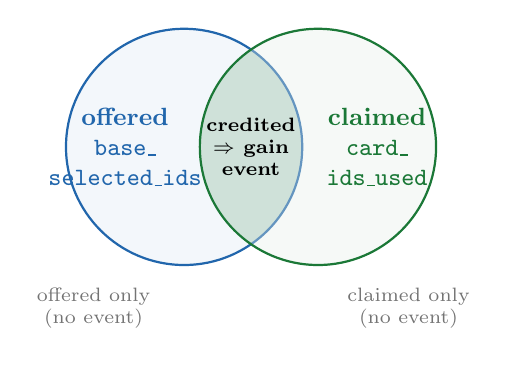
\begin{tikzpicture}[font=\small]
\begin{scope}
  \clip (0,0) circle (1.5);
  \fill[evgreen!45] (1.7,0) circle (1.5);
\end{scope}
\draw[cardblue, thick, fill=cardblue!10, fill opacity=0.55] (0,0) circle (1.5);
\draw[evgreen, thick, fill=evgreen!12, fill opacity=0.35] (1.7,0) circle (1.5);
\node[align=center, cardblue] at (-0.75,0)
  {\textbf{offered}\\{\scriptsize \code{base\_}}\\{\scriptsize \code{selected\_ids}}};
\node[align=center, evgreen] at (2.45,0)
  {\textbf{claimed}\\{\scriptsize \code{card\_}}\\{\scriptsize \code{ids\_used}}};
\node[align=center, font=\scriptsize\bfseries] at (0.85,0) {credited\\$\Rightarrow$ gain\\event};
\node[align=center, font=\scriptsize, text=black!55] at (-1.15,-2.05)
  {offered only\\(no event)};
\node[align=center, font=\scriptsize, text=black!55] at (2.85,-2.05)
  {claimed only\\(no event)};
\end{tikzpicture}
\caption{Gain attribution. A card is credited for a child only in the
intersection --- selected by the reader for that base parent \emph{and} declared
used by the mutator.}
\label{fig:attribution}
\end{figure}

\subsection{The gain value: base-relative, orientation-corrected}

The event's numeric payload is the child's fitness improvement over its base
parent, always expressed so that \emph{positive means better}:
\[
  \gain \;=\;
  \begin{cases}
     f(x) - f(\text{base}) & \text{if the metric is maximize},\\[2pt]
     f(\text{base}) - f(x) & \text{if the metric is minimize.}
  \end{cases}
\]
The orientation flip (\code{higher\_is\_better}) means every downstream comparison
--- ``was this a win?'' ($\gain \ge 0$) versus ``a loss?'' ($\gain < 0$) --- is
metric-agnostic. A minimize task and a maximize task feed the identical reputation
math.

\paragraph{Invalid children.} If the child failed to evaluate (invalid), the card
receives one \emph{forced-harm} event: $\gain=0.0$ with \code{invalid=True}. This
is counted as a harm below (Section~\ref{sec:harm}) --- a card that keeps
producing broken children is penalised even though its numeric delta is nominally
zero.

\subsection{Events are authoritative, not incremental}

Gain events are a \emph{pure function of the whole program pool}. On every write
sweep the updater (\code{CardStatsUpdater}) recomputes them from scratch and
restamps them onto the cards --- never accumulated. This makes reputation
deterministic and replayable: the same pool always yields the same events, and a
re-evaluation of an old child cannot double-count.

\section{Reputation: from gain events to a posterior}
\label{sec:rep}

Reputation collapses a card's event list into a \code{CardStatsBlock}
(\code{read/reputation.py}, \code{block\_from\_events} $\to$
\code{beta\_binomial\_posterior}). The model is a \textbf{Beta--Binomial downside
posterior}: it asks not ``how big is the average gain'' but ``how confident are we
this card is not a net source of harm.''

\subsection{Counting harms (the sign test)}
\label{sec:harm}

Partition the card's events. Let the \emph{finite valid} gains be
$\gain_1,\dots,\gain_m$ (invalid events excluded; non-finite values dropped), and
let $v$ be the number of \code{invalid} events. Define
\[
  n \;=\; m + v,
  \qquad
  k \;=\; \underbrace{\bigl|\{\, i : \gain_i < 0 \,\}\bigr|}_{\text{losses}}
          \;+\; \underbrace{v}_{\text{invalids}} .
\]
$k$ is the \emph{harm count}: a strict sign test. Any event whose gain is
\emph{below zero} counts as one harm; any invalid child counts as one harm; a win
($\gain \ge 0$) never counts. There is no per-card noise band and no threshold
other than zero.\footnote{The strict sign test is chosen for two properties. It is
\emph{monotone}: adding a winning event never changes any other event's verdict, so
more evidence only sharpens the count. And it is correct on a uniformly-harmful
card: every loss is counted, so a card that only ever hurt cannot read as
net-helpful. Eval noise is absorbed downstream by the counting posterior itself
(Section~\ref{sec:harmful}) --- the width of the Beta credible interval --- not by
any threshold on the raw gains.}

\begin{figure}[ht]
\centering
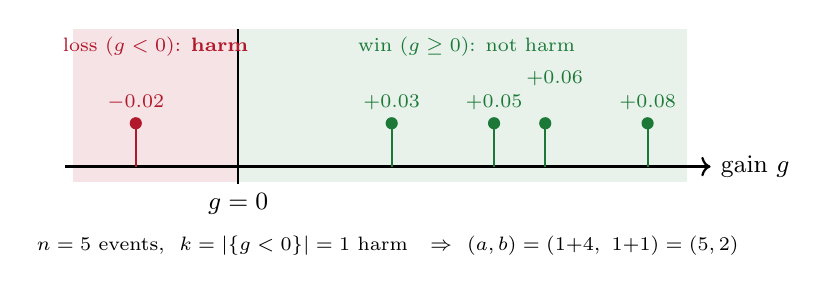
\begin{tikzpicture}[font=\small]
\fill[harmred!12] (-2.1,-0.2) rectangle (0,1.75);
\fill[evgreen!10] (0,-0.2) rectangle (5.7,1.75);
\draw[->,thick] (-2.2,0) -- (6.0,0) node[right]{gain $g$};
\draw[thick] (0,-0.22) -- (0,1.75);
\node[below] at (0,-0.22) {$g=0$};
\node[harmred, font=\scriptsize] at (-1.05,1.52) {loss ($g<0$): \textbf{harm}};
\node[evgreen, font=\scriptsize] at (2.9,1.52) {win ($g\ge 0$): not harm};
\foreach \x/\c in {-1.3/harmred, 1.95/evgreen, 3.25/evgreen, 3.9/evgreen, 5.2/evgreen}{
  \draw[\c, thick] (\x,0) -- (\x,0.55);
  \fill[\c] (\x,0.55) circle (2.2pt);
}
\node[harmred, font=\scriptsize] at (-1.3,0.82) {$-0.02$};
\node[evgreen, font=\scriptsize] at (1.95,0.82) {$+0.03$};
\node[evgreen, font=\scriptsize] at (3.25,0.82) {$+0.05$};
\node[evgreen, font=\scriptsize] at (4.02,1.12) {$+0.06$};
\node[evgreen, font=\scriptsize] at (5.2,0.82) {$+0.08$};
\node[align=center, font=\scriptsize] at (1.9,-1.0)
  {$n=5$ events,\ \ $k=\lvert\{g<0\}\rvert=1$ harm
   \ \ $\Rightarrow$\ \ $(a,b)=(1{+}4,\ 1{+}1)=(5,2)$};
\end{tikzpicture}
\caption{The harm count is a strict sign test. The helpful card of
Section~\ref{sec:worked}: five gains, one below zero, so $k=1$. A win never
counts as harm and never moves another event's verdict --- the sign test is
monotone, and it counts every loss on a card that only ever hurt.}
\label{fig:signtest}
\end{figure}

\subsection{The downside posterior}

Treat the $n$ events as Bernoulli trials with a latent ``help probability''
$\theta$, and place a uniform $\Beta(1,1)$ prior on it. Observing $k$ harms out of
$n$ gives the posterior
\[
  \theta \;\sim\; \Beta(a,b),
  \qquad
  a \;=\; 1 + (n-k),
  \qquad
  b \;=\; 1 + k .
\]
So $a-1$ counts non-harmful outcomes and $b-1$ counts harms. From this single
posterior every scalar the system uses is derived:
\begin{align}
  \text{\code{p\_help\_mean}} \;\;\mu &= \frac{a}{a+b}, \\[4pt]
  \text{\code{p\_help\_lo20}} \;\;\ell &= F^{-1}_{\Beta(a,b)}(q_{\text{lo}}),
    \qquad q_{\text{lo}} = \text{\code{confident\_quantile}} = 0.20, \\[4pt]
  \text{\code{efficacy\_confident}} &=
    \bigl[\, n>0 \,\wedge\, \ell > \tau_{\text{c}} \,\wedge\, M > 0 \,\bigr],
    \qquad \tau_{\text{c}} = \text{\code{confident\_threshold}} = 0.5 .
\end{align}
$\mu$ is the point estimate of help-probability; $\ell$ is a \emph{pessimistic}
lower bound (the 20th percentile of the posterior --- we only call a card
``confident'' if even the unlucky tail clears one-half). \code{efficacy\_confident}
additionally requires a strictly positive magnitude, so a card whose median effect
is zero can never read as a confident win. Figure~\ref{fig:beta} shows how the same
$(a,b)$ machinery places helpful, weak, and cold cards relative to the baseline.

\begin{figure}[ht]
\centering
\includegraphics[width=0.86\textwidth]{memrep_beta.pdf}
\caption{Every card is a $\Beta(a,b)$ posterior over its help-probability
$\theta$. A helpful card ($\Beta(5,2)$) sits to the right of the $\Beta(3,3)$
baseline arm; a weak/harmful card ($\Beta(2,4)$) to its left; a cold card
($\Beta(1,1)$) is flat (maximal uncertainty). Shaded: the pessimistic lower-20\%
tail of the helpful posterior --- because its bound $\ell=0.578$ clears
$\tau_c=0.5$, the card reads as \code{efficacy\_confident}.}
\label{fig:beta}
\end{figure}

\subsection{Magnitude}

The posterior says \emph{how reliably} a card helps; the magnitude says \emph{how
much}. It is the median of the finite gains (\code{IntroGain\_best\_median}):
\[
  M \;=\; \operatorname{median}(\gain_1,\dots,\gain_m)
  \qquad (\,M = 0 \text{ if there are no finite gains}\,).
\]
Crucially $M$ is \textbf{signed}: a card whose gains are mostly negative has a
negative median, and that sign propagates into the bid (Section~\ref{sec:ev}),
where it makes the card bid \emph{against} its own injection.

\subsection{Cold cards}

A card with no events yields no block. The reputation model
(\code{BetaBinomialReputation}) then falls back to the \emph{cold prior}
\[
  (a,b) = \text{\code{cold\_prior}} = (1,1), \qquad M = \text{None},
\]
i.e.\ a uniform posterior --- maximal uncertainty, neither endorsed nor condemned.
The auction supplies the missing magnitude by \emph{borrowing} a gain scale from
the round (Section~\ref{sec:ev}) --- the warm cards' median positive gain, or the
task's declared significant-change threshold --- which is what gives never-tried
cards a fair, task-scaled shot at exploration.

\section{BD-proximity reputation (context-local variant)}
\label{sec:bd}

\code{BDProximityReputation} is a drop-in reputation model that makes a card's
reputation \emph{query-dependent}. At read time it snapshots the current
MAP-Elites tessellation (\code{behavior\_space.model\_copy(deep=True)}), finds the
cell of the query parent, and re-buckets the card's gain events, keeping only those
whose \emph{own} parent fell in that same cell. It then runs the identical
Beta--Binomial math on the in-cell subset. If the cell is cold (no in-cell events)
it delegates to a global \code{fallback} \code{BetaBinomialReputation}.

The effect: a card is judged by how it performed \emph{on parents like the one we
are about to mutate}, not by its global average. This requires a single-island
algorithm that exposes a top-level \code{behavior\_space} for the config's
\code{\$\{ref:behavior\_space\}} to bind to; a \code{multi\_island} algorithm has
per-island spaces and no top-level one, so the pairing is caught at config time by
\code{validate\_reputation\_island\_compat}, which raises \code{NotImplementedError}
rather than let the ref silently bind to nothing.

\paragraph{A one-line example.} Suppose card $C$ has ten gain events, but only three
of them came from parents that land in the query parent's current cell, and those
three read $\{+0.04, -0.01, +0.03\}$. The global model would score $C$ on all ten;
BD-proximity scores it on just those three --- $n=3$, $k_{\text{harm}}=1$, so the
downside posterior is $\Beta(1+2,\,1+1)=\Beta(3,2)$ and $\hat M$ is the median of
that in-cell triple. If instead \emph{zero} events fell in the cell, \code{\_in\_cell}
returns \code{None} and the whole judgment delegates to the global \code{fallback} ---
the cell is simply too cold to have a local opinion.

\section{Expected value and the bid}
\label{sec:ev}

The EV auctioneer (\code{EVThompsonAuctioneer}, arm \code{thompson\_ev}) converts a
candidate's $(a,b,M)$ into a single realized \emph{bid} via one Thompson draw:
\[
  \tilde\theta \sim \Beta(a,b),
  \qquad
  \hat M = \begin{cases} M & M \text{ known} \\
                         M_{\text{cold}} & M \text{ unknown (cold)} \end{cases},
  \qquad
  \text{bid} \;=\; \tilde\theta \cdot \hat M .
\]
The bid is a sampled expected value: a reliability draw $\tilde\theta \in (0,1)$
scaled by the effect size $\hat M$. For a warm card $\hat M$ is its own signed
median gain; a cold card has no gain scale of its own, so it \emph{borrows} one.

\paragraph{The borrowed cold magnitude.} $M_{\text{cold}}$ is chosen once per round,
in this order of preference:
\begin{enumerate}[nosep, leftmargin=1.7em]
  \item \textbf{warm median} --- the median of the \emph{positive} magnitudes of the
        warm cards on the same shortlist. This is the task's own realized
        helpful-gain scale: ``a card that helps here is worth about this much.''
  \item \textbf{declared threshold} --- if the round has no warm magnitude to borrow,
        the primary metric's \code{significant\_change} (from the shared
        \code{metrics\_context}), a task-declared meaningful-gain threshold in the
        \emph{same units} as $M$.
  \item \textbf{inert unit} --- only if the round is all-cold \emph{and} the task
        declares no \code{significant\_change}: a placeholder $M_{\text{cold}}=1$.
        Being then a common positive factor across every cold bid, it cancels from
        the budgeter's ranking and clears the zero floor for any card --- it sets no
        real scale, it just keeps cold cards explorable.
\end{enumerate}
So a cold card's exploration bid tracks the gains cards actually earn on this task,
not a fixed scale-blind constant. Two consequences fall straight out of the signs:
\begin{itemize}[nosep]
  \item A \textbf{proven-harmful} card has $M<0$, so every bid is negative and is
        killed by the EV floor below --- the system abstains rather than injecting
        a known-bad card.
  \item A \textbf{cold} card bids $\tilde\theta \cdot M_{\text{cold}}$ with
        $\tilde\theta \sim \Beta(1,1) = \mathrm{Uniform}(0,1)$: a strictly positive,
        high-variance bid at the borrowed scale. This is the exploration term.
\end{itemize}

Figure~\ref{fig:bid} shows the three resulting bid distributions and why the sign
of $M$ is doing the safety work.

\begin{figure}[ht]
\centering
\includegraphics[width=0.86\textwidth]{memrep_bid.pdf}
\caption{Realized bids $\tilde\theta\cdot\hat M$ for three card types. A harmful
card ($M=-0.075$) lands entirely in the \emph{abstain} region (bid $\le\phi=0$) and
can never be injected; a helpful card ($M=+0.05$) concentrates on a modest positive
bid; a cold card spreads uniformly over its \emph{borrowed} scale --- here the lone
positive warm magnitude, $M_{\text{cold}}={+}0.05$ --- pure exploration.}
\label{fig:bid}
\end{figure}

\section{The auction}
\label{sec:auction}

\subsection{Thompson EV auction (the shipped arm)}

Each candidate is evaluated independently against a virtual ``inject nothing''
baseline arm. Per candidate the auctioneer draws a fresh gate sample and a
baseline sample:
\[
  \theta \sim \Beta(a,b),
  \qquad
  \theta_0 \sim \Beta(\alpha_0,\beta_0),
  \qquad (\alpha_0,\beta_0) = \text{\code{baseline\_prior}} = (3,3),
\]
and the candidate \textbf{wins} iff
\[
  \boxed{\;\theta > \theta_0 \;\;\wedge\;\; \text{bid} > \phi\;}
  \qquad \phi = \text{\code{ev\_floor}} = 0.0 .
\]
The first clause is a Thompson-sampling comparison: the card must, on this draw,
look more reliable than a coin the baseline ``believes'' is about $0.5$
($\Beta(3,3)$ has mean $0.5$ but is concentrated, so a card needs a genuinely
strong posterior to beat it often). The second clause is the EV gate: even a
reliable-looking card is dropped if its realized bid is not positive, which is
exactly how negative-magnitude (harmful) cards are excluded.

\paragraph{Why a $\Beta(3,3)$ baseline.} The baseline arm encodes ``the prompt is
already fine; injecting nothing is a solid default.'' Its concentration at $0.5$
means marginal cards lose most of the time while strongly-endorsed cards win most
of the time, and cold cards land near a coin flip --- exploration without
recklessness (Figure~\ref{fig:winprob}).

\begin{figure}[ht]
\centering
\includegraphics[width=0.82\textwidth]{memrep_winprob.pdf}
\caption{Chance of clearing the reliability gate, $\Pr(\theta>\theta_0)$ with
$\theta_0\sim\Beta(3,3)$, by card strength. A strongly-endorsed card wins most
draws; a cold card is a coin flip (pure exploration); a weak card is filtered out
most of the time. These are exact quadratures, not the median.}
\label{fig:winprob}
\end{figure}

\paragraph{Draw order is pinned.} For seed-exact replay the RNG is consumed in a
fixed order: \emph{all} bid draws first (one $\tilde\theta$ per candidate), then
per candidate the gate $\theta$ followed by the baseline $\theta_0$. Re-running the
auction with the same seed and same candidate list reproduces the same winners
exactly.

\subsection{Safety auction (the alternative arm)}

\code{ThompsonAuctioneer} (arm \code{thompson}) is the magnitude-free variant: it
keeps only the reliability gate,
\[
  \theta \sim \Beta(a,b), \quad \theta_0 \sim \Beta(3,3), \quad
  \text{win} \iff \theta > \theta_0,
\]
with no bid and no EV floor. It pairs with \code{TopThetaBudgeter} and is used when
effect \emph{size} should not influence selection --- only proven reliability.

\section{Budget: capping winners to the injection slot}

The auction can return several winners; the injection budget is one
(\code{reader.max\_cards} $=1$). The budgeter enforces it:
\begin{itemize}[nosep]
  \item \code{TopBidBudgeter} (EV arm) --- keeps the \code{max\_cards} winners with
        the highest realized \emph{bid}.
  \item \code{TopThetaBudgeter} (safety arm) --- keeps the highest realized
        \emph{gate} $\theta$.
\end{itemize}
Both are no-ops when the number of winners already fits the budget, preserving
auction order. So the final decision is: of the cards that beat ``inject nothing''
on this draw, inject the single strongest by its \emph{realized} draw (the bid
$\tilde\theta\hat M$ under the EV arm, the gate $\theta$ under the safety arm) ---
or, if none beat the baseline, inject nothing.

\section{One parent, the whole shortlist: a per-card auction round}
\label{sec:round}

The previous sections followed a \emph{single} card. In a real read, one parent
program~$P$ retrieves a \emph{shortlist} of up to ten cards, and every card runs
the \S\ref{sec:rep}--\S\ref{sec:ev} machinery \emph{independently}: each has its own
gain-event history, so each gets its own posterior $\Beta(a,b)$, its own magnitude
$\hat M$, and thus its own expected value $\mathrm{EV}=\mu\cdot\hat M$ (a summary; the
auction samples rather than using this number directly). The auction then draws each
card against the \emph{same} baseline arm and the budget keeps the single selection
with the highest \emph{realized} bid $\tilde\theta\hat M$. Figure~\ref{fig:round}
shows the fan-out for one parent with four shortlisted cards; Table~\ref{tab:round}
gives the exact arithmetic behind each box.

\begin{figure}[H]
\centering
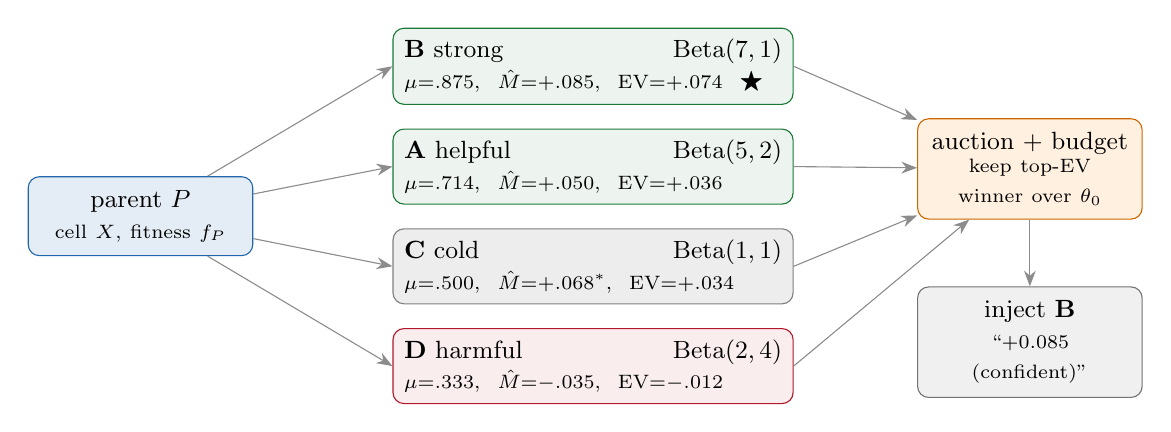
\begin{tikzpicture}[font=\small,
  card/.style={draw, rounded corners, align=left, inner sep=4pt, text width=48mm,
               minimum height=8mm},
  hub/.style={draw, rounded corners, align=center, inner sep=5pt, text width=25mm},
  a/.style={-{Stealth[length=2mm]}, draw=black!45}]
\node[card, fill=evgreen!8, draw=evgreen] (B)
  {\textbf{B} strong \hfill $\Beta(7,1)$\\
   {\scriptsize $\mu{=}.875$,\ \ $\hat M{=}{+}.085$,\ \ EV${=}{+}.074$}\ \ \textbf{$\bigstar$}};
\node[card, fill=evgreen!8, draw=evgreen, below=3mm of B] (A)
  {\textbf{A} helpful \hfill $\Beta(5,2)$\\
   {\scriptsize $\mu{=}.714$,\ \ $\hat M{=}{+}.050$,\ \ EV${=}{+}.036$}};
\node[card, fill=coldgray!14, draw=coldgray, below=3mm of A] (C)
  {\textbf{C} cold \hfill $\Beta(1,1)$\\
   {\scriptsize $\mu{=}.500$,\ \ $\hat M{=}{+}.068^{*}$,\ \ EV${=}{+}.034$}};
\node[card, fill=harmred!8, draw=harmred, below=3mm of C] (D)
  {\textbf{D} harmful \hfill $\Beta(2,4)$\\
   {\scriptsize $\mu{=}.333$,\ \ $\hat M{=}{-}.035$,\ \ EV${=}{-}.012$}};
\coordinate (Lmid) at ($(B.west)!0.5!(D.west)$);
\coordinate (Rmid) at ($(B.east)!0.5!(D.east)$);
\node[hub, fill=cardblue!12, draw=cardblue] (P) at ($(Lmid)+(-32mm,0)$)
  {parent $P$\\{\scriptsize cell $X$, fitness $f_P$}};
\node[hub, fill=orange!12, draw=orange!80!black] (bud) at ($(Rmid)+(30mm,6mm)$)
  {auction $+$ budget\\{\scriptsize keep top-EV\\ winner over $\theta_0$}};
\node[hub, fill=black!6, draw=black!55] (out) at ($(bud)+(0,-22mm)$)
  {inject \textbf{B}\\{\scriptsize ``$+0.085$ (confident)''}};
\draw[a] (P)--(B.west); \draw[a] (P)--(A.west);
\draw[a] (P)--(C.west); \draw[a] (P)--(D.west);
\draw[a] (B.east)--(bud); \draw[a] (A.east)--(bud);
\draw[a] (C.east)--(bud); \draw[a] (D.east)--(bud);
\draw[a] (bud)--(out);
\end{tikzpicture}
\caption{One parent's shortlist. Each card independently forms its own posterior
and expected value; the auction draws them against a shared $\Beta(3,3)$ baseline
and the budget injects the single winner with the highest \emph{realized} bid
($\bigstar$~=~B on a typical draw; the EV column orders them but the draw decides). A cold card
(C) rides the $\mu{=}0.5$ exploration coin-flip on a \emph{borrowed} magnitude
($^{*}$~=~median of the positive warm gains,
$\operatorname{median}(.085,.050){=}.068$); a harmful card (D) has $\mathrm{EV}<0$
and abstains regardless of its gate draw.}
\label{fig:round}
\end{figure}

\begin{table}[H]
\centering
\footnotesize
\begin{tabular}{@{}llcccccc l@{}}
\toprule
Card & $(n,k)$ & $\Beta(a,b)$ & $\mu$ & $\ell_{20}$ & $\hat M$ & EV${=}\mu\hat M$ & $\Pr(\theta{>}\theta_0)$ & decision on this draw \\
\midrule
\textbf{B} strong  & $(6,0)$ & $\Beta(7,1)$ & $0.875$ & $0.795$ & $+0.085$ & $+0.074$ & $0.955$ & selected --- \textbf{winner} \\
\textbf{A} helpful & $(5,1)$ & $\Beta(5,2)$ & $0.714$ & $0.578$ & $+0.050$ & $+0.036$ & $0.803$ & selected (loses budget) \\
\textbf{C} cold    & $(0,0)$ & $\Beta(1,1)$ & $0.500$ & $0.200$ & $+0.068^{*}$ & $+0.034$ & $0.500$ & explores ($\approx$coin flip) \\
\textbf{D} harmful & $(4,3)$ & $\Beta(2,4)$ & $0.333$ & $0.169$ & $-0.035$ & $-0.012$ & $0.262$ & abstains (bid $<\phi$) \\
\bottomrule
\end{tabular}
\caption{Exact per-card arithmetic for Figure~\ref{fig:round}. $n$ valid events,
$k$ of them losses $\Rightarrow a{=}1{+}(n{-}k),\,b{=}1{+}k$; $\mu{=}a/(a{+}b)$;
$\ell_{20}{=}F^{-1}_{\Beta}(0.20)$; $\hat M$ the signed median gain (or, for the
cold card, the borrowed warm-median magnitude
$0.068^{*}{=}\operatorname{median}(.085,.050)$); EV the \emph{expected} bid
$\mu\hat M$ (the realized
bid is one Thompson draw $\tilde\theta\hat M$); $\Pr(\theta{>}\theta_0)$ the exact
chance of beating the $\Beta(3,3)$ arm. A card is \emph{selected} iff its gate draw
beats the baseline \emph{and} its realized bid exceeds $\phi{=}0$; the budget
(\code{TopBidBudgeter}) then keeps the single selection with the highest
\emph{realized} bid $\tilde\theta\hat M$ --- \emph{not} the deterministic EV column,
which is shown only to order the cards by expectation. On a typical draw $B$'s bid
tops $A$'s, so $B$ wins and $A$ --- though also a legitimate selection --- is dropped;
on an unlucky draw $A$ could edge $B$. Both $A$ and $B$ satisfy
$\ell_{20}{>}0.5\wedge\hat M{>}0$, so both are \emph{confidence-eligible} --- only $B$
is \emph{rendered} as confident here because it takes the single slot.}
\label{tab:round}
\end{table}

The key point is \emph{independence and comparison}: the posterior and EV are
decided \emph{per card} from that card's own evidence (rows of Table~\ref{tab:round}
never interact), but \emph{selection} is a \emph{competition} --- the shared
$\Beta(3,3)$ gate and the one-slot budget mean a card's fate depends on the company
it keeps. $A$ is a perfectly good card that beats ``inject nothing'' four times in
five; it loses this round only because $B$'s six clean wins give it a higher
expected value for the single available slot.

\section{Rendering the endorsement}
\label{sec:render}

A budgeted winner is turned into prompt text by the renderer
(\code{read/render.py}). For an \textbf{exemplar program} card the renderer bypasses
the posterior block entirely and reads \code{card.fitness} directly (``exemplar
fitness $f$''); the reputation math never touches a program card's endorsement line.
For an \textbf{insight} card the efficacy line is gated on the
same \code{efficacy\_confident} flag from Section~\ref{sec:rep}:
\begin{itemize}[nosep]
  \item \code{efficacy\_confident} \emph{and} $M>0$: rendered as
        ``\emph{median improvement $+M$ (confident)}'';
  \item otherwise the median is non-positive or the posterior is not confident, and
        the endorsement is withheld / caveated.
\end{itemize}
Thus the prompt never advertises a confident improvement the posterior does not
support.

\section{Harm eviction (write side, for completeness)}
\label{sec:harmful}

The same posterior powers a \emph{separate} decision on the write side: whether to
\emph{delete} a card outright (\code{write/eviction.py}, \code{HarmEvictor} via the
\code{CardScorer} Protocol). A card is \code{is\_confidently\_harmful} iff
\[
  n \ge \text{\code{harm\_min\_events}} = 3
  \quad\wedge\quad
  F^{-1}_{\Beta(a,b)}\bigl(q_{\text{h}}\bigr) < \tau_{\text{h}},
  \qquad q_{\text{h}}=0.80,\;\; \tau_{\text{h}}=0.5 .
\]
This is the mirror image of \code{efficacy\_confident}: it demands at least three
events and then checks an \emph{optimistic} upper quantile (the 80th percentile of
the help-posterior). Only if even that optimistic bound falls below one-half ---
i.e.\ the card is harmful under a generous reading --- is it evicted. This is where
symmetric eval noise is absorbed: a card whose losses and wins roughly cancel keeps
$\mu \approx 0.5$ and is never flagged, while a consistent downward bias is.
Note this flag is consulted \emph{only} by the evictor; the read auction never
calls it. The companion write-side report (\emph{``How a Run Becomes a Card''}, \S8)
covers eviction end-to-end --- the harm-event bookkeeping, the throttled
consolidation it competes with, and why the evictor consumes this posterior through
a Protocol rather than importing the reader.

\section{Two worked examples}
\label{sec:worked}

\paragraph{A helpful card.} Gains $(\,+0.05,\,+0.03,\,+0.08,\,-0.02,\,+0.06\,)$,
no invalids. One gain is below zero, so $n=5$, $k=1$, giving
$(a,b)=(5,2)$. Then
\[
  \mu = \tfrac{5}{7} = 0.714,\quad
  \ell = F^{-1}_{\Beta(5,2)}(0.20) = 0.578,\quad
  M = \operatorname{median} = 0.05 .
\]
Since $\ell = 0.578 > 0.5$ and $M>0$, \code{efficacy\_confident} is \textbf{true} ---
the renderer would advertise ``median improvement $+0.05$ (confident).'' In the EV
auction this card draws $\theta \sim \Beta(5,2)$ (mean $0.71$) against
$\theta_0 \sim \Beta(3,3)$, winning the gate about \textbf{80\%} of the time, with a
positive bid.

\paragraph{A harmful card.} Gains $(\,-0.10,\,-0.20,\,-0.05,\,+0.01\,)$. Three are
below zero, so $n=4$, $k=3$, giving $(a,b)=(2,4)$. Then
\[
  \mu = \tfrac{2}{6} = 0.333,\quad
  F^{-1}_{\Beta(2,4)}(0.80) = 0.490 < 0.5,\quad
  M = \operatorname{median} = -0.075 .
\]
With $n \ge 3$ and the optimistic 80th-percentile bound below $0.5$, the card is
\code{is\_confidently\_harmful} $\Rightarrow$ \textbf{evicted}. Even if it survived
to an auction, its magnitude is negative, so every bid $\tilde\theta \cdot (-0.075)$
is negative and fails the EV floor: it can never be injected.

\paragraph{A cold card.} No events: $(a,b)=(1,1)$, $M$ unknown. Its gate draw
$\theta \sim \mathrm{Uniform}(0,1)$ beats $\theta_0 \sim \Beta(3,3)$ almost exactly
\textbf{50\%} of the time --- a fair coin for exploration. Its bid magnitude is
\emph{borrowed} from the round (\S\ref{sec:ev}): the median positive gain of the
warm cards sharing its shortlist, so a never-tried card explores at the same scale
the task's proven cards deliver. (For contrast, a weak card with posterior
$\Beta(2,4)$ wins the gate only about \textbf{26\%} of the time.)

\section{Parameter reference}

\begin{center}
\begin{longtable}{@{}lll@{}}
\toprule
Symbol / flag & Config key & Default \\
\midrule
\endhead
Beta prior on help-probability & (fixed) & $\Beta(1,1)$ \\
Cold-card posterior            & \code{reputation.cold\_prior}       & $(1,1)$ \\
Confident lower quantile $q_{\text{lo}}$ & \code{reputation.confident\_quantile} & $0.20$ \\
Confident threshold $\tau_{\text{c}}$    & \code{reputation.confident\_threshold} & $0.5$ \\
Harm min.\ events              & \code{reputation.harm\_min\_events} & $3$ \\
Harm quantile $q_{\text{h}}$   & \code{reputation.harm\_quantile}    & $0.80$ \\
Harm threshold $\tau_{\text{h}}$ & \code{reputation.harm\_threshold} & $0.5$ \\
Baseline (no-card) arm prior   & \code{auction.baseline\_prior}      & $(3,3)$ \\
Cold-card magnitude $M_{\text{cold}}$ & \emph{borrowed: warm median $\to$ \code{significant\_change}} & --- \\
EV floor $\phi$                & \code{auction.ev\_floor}            & $0.0$ \\
Retrieval fan-out              & \code{research.default\_top\_k}     & $10$ \\
Recall shortlist width         & \code{research.max\_cards}          & $10$ \\
Injection budget               & \code{reader.max\_cards}            & $1$ \\
\bottomrule
\end{longtable}
\end{center}

\paragraph{One-line summary.} Each card's history of measured effects becomes a
Beta downside posterior (how reliably it helps) and a signed median magnitude (how
much); the two multiply into a sampled expected value that must beat both a
$\Beta(3,3)$ ``inject nothing'' baseline and a zero EV floor; at most one winner
per mutation is rendered, and only with a confidence-gated endorsement.

\end{document}
